\begin{figure}[H]
\centering
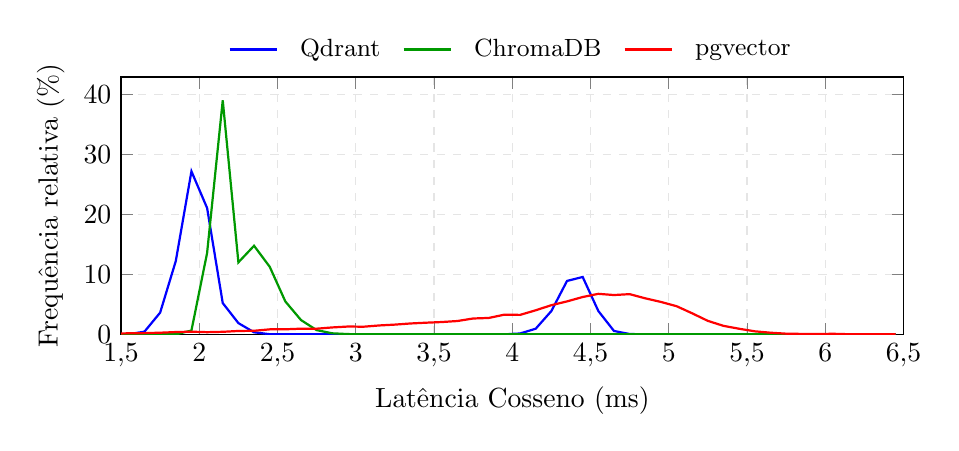
\begin{tikzpicture}
\begin{axis}[
    width=0.95\textwidth, height=0.40\textwidth,
    xlabel={Latência Cosseno (ms)}, ylabel={Frequência relativa (\%)},
    xmin=1.5, xmax=6.5, ymin=0,
    grid=major, grid style={dashed, gray!20},
    /pgf/number format/use comma,
    legend columns=3,
    legend style={at={(0.5,1.02)}, anchor=south, font=\small, draw=none, /tikz/column sep=6pt}
]
\addplot[color=blue, thick, mark=none] coordinates {
    (1.45, 0.00) (1.55, 0.02) (1.65, 0.45) (1.75, 3.62) (1.85, 12.22) (1.95, 27.17) (2.05, 21.06) (2.15, 5.21) (2.25, 1.87) (2.35, 0.34) (2.45, 0.02) (2.55, 0.01) (2.65, 0.01) (2.75, 0.01) (2.85, 0.00) (2.95, 0.01) (3.05, 0.00) (3.15, 0.00) (3.25, 0.00) (3.35, 0.00) (3.45, 0.00) (3.55, 0.00) (3.65, 0.00) (3.75, 0.01) (3.85, 0.00) (3.95, 0.00) (4.05, 0.14) (4.15, 0.94) (4.25, 3.89) (4.35, 8.90) (4.45, 9.56) (4.55, 3.89) (4.65, 0.56) (4.75, 0.05) (4.85, 0.01) (4.95, 0.00) (5.05, 0.00) (5.15, 0.00) (5.25, 0.00) (5.35, 0.00) (5.45, 0.00) (5.55, 0.00) (5.65, 0.00) (5.75, 0.00) (5.85, 0.00) (5.95, 0.00) (6.05, 0.00) (6.15, 0.00) (6.25, 0.00) (6.35, 0.00) (6.45, 0.00)
};
\addlegendentry{Qdrant}
\addplot[color=green!60!black, thick, mark=none] coordinates {
    (1.45, 0.00) (1.55, 0.00) (1.65, 0.00) (1.75, 0.00) (1.85, 0.00) (1.95, 0.63) (2.05, 13.56) (2.15, 39.00) (2.25, 12.00) (2.35, 14.76) (2.45, 11.27) (2.55, 5.48) (2.65, 2.38) (2.75, 0.70) (2.85, 0.17) (2.95, 0.04) (3.05, 0.01) (3.15, 0.00) (3.25, 0.00) (3.35, 0.00) (3.45, 0.00) (3.55, 0.00) (3.65, 0.00) (3.75, 0.00) (3.85, 0.00) (3.95, 0.00) (4.05, 0.00) (4.15, 0.00) (4.25, 0.00) (4.35, 0.00) (4.45, 0.00) (4.55, 0.00) (4.65, 0.00) (4.75, 0.00) (4.85, 0.00) (4.95, 0.00) (5.05, 0.00) (5.15, 0.00) (5.25, 0.00) (5.35, 0.00) (5.45, 0.00) (5.55, 0.00) (5.65, 0.00) (5.75, 0.00) (5.85, 0.00) (5.95, 0.00) (6.05, 0.00) (6.15, 0.00) (6.25, 0.00) (6.35, 0.00) (6.45, 0.00)
};
\addlegendentry{ChromaDB}
\addplot[color=red, thick, mark=none] coordinates {
    (1.45, 0.13) (1.55, 0.17) (1.65, 0.20) (1.75, 0.27) (1.85, 0.38) (1.95, 0.44) (2.05, 0.36) (2.15, 0.42) (2.25, 0.56) (2.35, 0.59) (2.45, 0.83) (2.55, 0.84) (2.65, 0.94) (2.75, 0.94) (2.85, 1.15) (2.95, 1.30) (3.05, 1.27) (3.15, 1.48) (3.25, 1.62) (3.35, 1.81) (3.45, 1.94) (3.55, 2.05) (3.65, 2.22) (3.75, 2.64) (3.85, 2.73) (3.95, 3.28) (4.05, 3.24) (4.15, 4.01) (4.25, 4.86) (4.35, 5.49) (4.45, 6.22) (4.55, 6.75) (4.65, 6.55) (4.75, 6.70) (4.85, 6.00) (4.95, 5.40) (5.05, 4.69) (5.15, 3.50) (5.25, 2.24) (5.35, 1.41) (5.45, 0.93) (5.55, 0.50) (5.65, 0.27) (5.75, 0.11) (5.85, 0.07) (5.95, 0.05) (6.05, 0.09) (6.15, 0.02) (6.25, 0.01) (6.35, 0.00) (6.45, 0.00)
};
\addlegendentry{pgvector}
\end{axis}
\end{tikzpicture}
\caption{Distribuição da latência para as consultas sequenciais sob a \textbf{Similaridade de Cosseno}, agregando as \num{50000} consultas das 5 réplicas de cada motor (classes de 0,1~ms). Menos de 0,5\% das consultas, todas do pgvector e abaixo de 1,5~ms, ficam fora da janela representada.}
\label{fig:latencia_distribuicao_cosine}
\end{figure}
